%----------------------------------------------------------------------------------------------------------------------

\begin{frame}{Why Feature Generalization?}

\begin{columns}[T]
\column{0.7\linewidth}
\begin{itemize}[noitemsep,label=\textbullet,topsep=2pt,parsep=2pt,partopsep=2pt]
\item Many commercial CAD applications model using Features
\item Features reflect terminologies used 
\item Shape same but {\em feature}-nomenclature, usage, different
\item {\em Box}, {\em Pad}, {\em Protrusion}, {\em Extrude}, But the same shape. 
\item Problems in 
	\begin{itemize}[noitemsep,label=\textbullet,topsep=2pt,parsep=2pt,partopsep=2pt]
	\item Learning a new CAD system
	\item Interoperability between different CAD applications
	\item Development of functionality for downstream applications
	\end{itemize}
\item Need a neutral way of defining {\em form features}
\end{itemize}

\column{0.3\linewidth}

	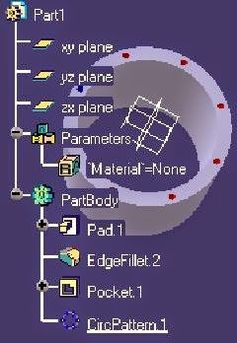
\includegraphics[width=0.8\linewidth]{../Common/images/CatiaFeatures.jpg}
	
	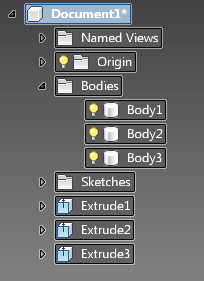
\includegraphics[width=0.8\linewidth]{../Common/images/InventorFeatures}

\end{columns}



\end{frame}

%----------------------------------------------------------------------------------------------------------------------

\begin{frame}{Spatial Grammars}

\begin{itemize}[noitemsep,label=\textbullet,topsep=2pt,parsep=2pt,partopsep=2pt]
\item Spatial Grammars = \{Graph-Shape-Set Grammars etc.\} 
\item Aim: Formalism through terse but expressive definitions
\item Shape Grammar in a generative approach
\item Formally introduced by Stiny and Gips \cite{Stiny1971} 
\item Primarily used for exploratory, evolutionary design process. 
\item Hoisl et. al.\cite{Hoisl2009} used Primitives, {\em Sweeping} and Booleans
\item Limited work in CAD, especially Feature Based CAD.

\end{itemize}

\begin{center}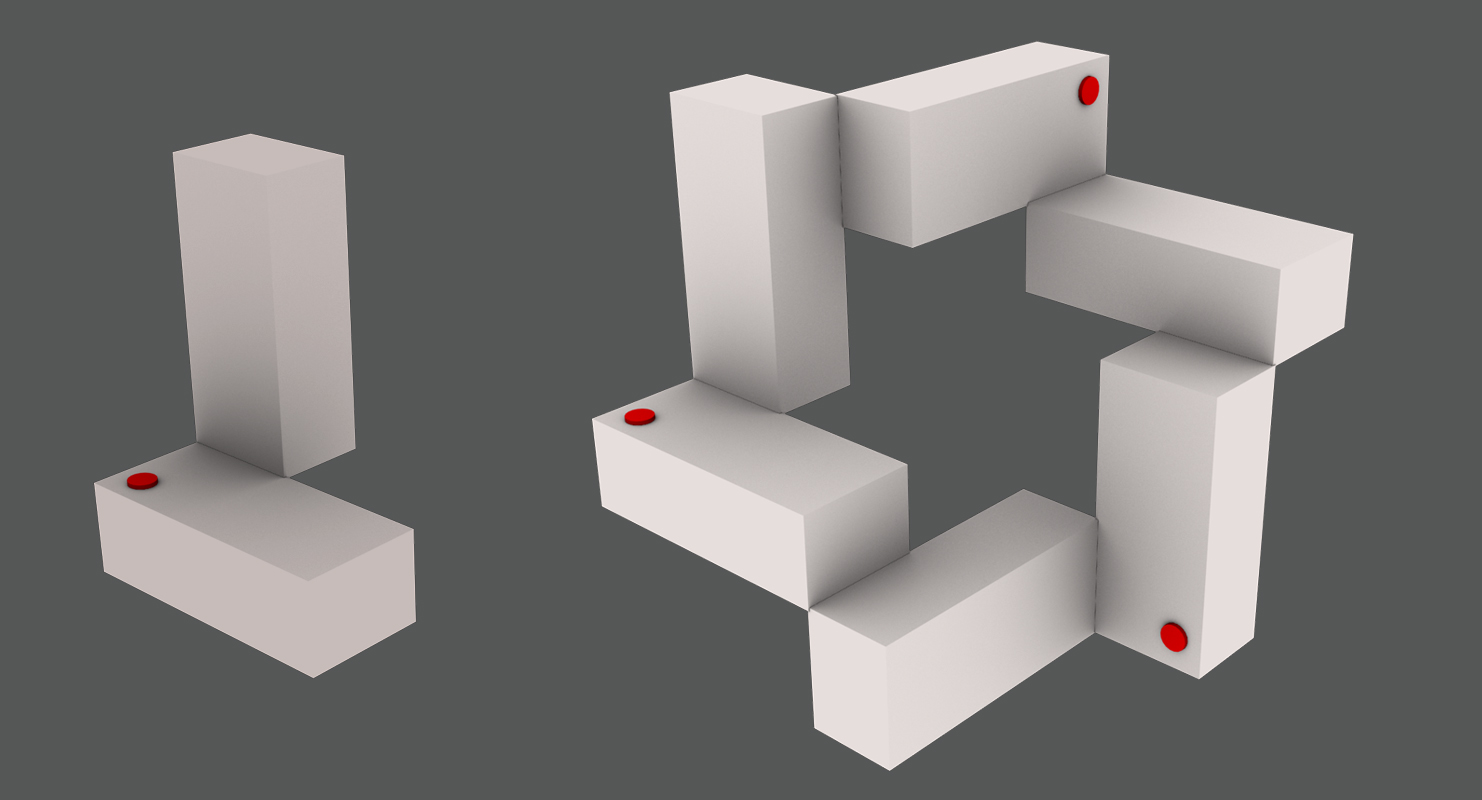
\includegraphics[width=0.6\linewidth]{../Common/images/SpatialGrammar.jpg}\end{center}


\end{frame}

%----------------------------------------------------------------------------------------------------------------------